\section{子研究一:各人格特质的广告文案特征分析} 
\label{study3-substudy1}

\subsection{方法}
\label{LIWC}

\textbf{(1)实验材料}

在本研究的研究一与研究二中,共收集了145条基于大五人格模型(外倾性、开放性、尽责性、宜人性、神经质)定制生成的广告文案,覆盖了高水平与低水平人格特质的广告版本。然而,统计结果显示,145条广告中仅有8条为针对低水平特质设计的广告,样本量严重不足,难以对低水平特质的广告特征进行系统性分析。因此,为确保分析结果的科学性与代表性,当前聚焦于137条针对高水平人格特质(即高外倾、高开放、高尽责、高宜人和高神经质)设计的广告文案,通过定量文本分析深入探索不同人格特质广告文案的语言特征及其潜在模式。

\textbf{(2)分析方法}

本研究采用语言分析与词汇计算软件(Linguistic Inquiry and Word Count, LIWC)对137条广告文案进行文本特征分析。LIWC 是一款广泛应用于语言心理学、社会科学和计算传播学等领域的文本分析工具,由 Pennebaker 等人开发 \citep{pennebaker2007linguistic}。该工具通过内置的词典库对文本进行分类和统计,能够揭示文本的心理、情感及语言特征,其核心优势在于对语言风格和心理状态的多维度解析。LIWC 词库结构丰富,包含多个心理、情感和语言类别,涵盖数千个词根和语言表述单元。其分析维度包括但不限于情感类别、认知过程、社会过程和驱动因素等。情感类别包括正面情感(positive emotion)和负面情感(negative emotion),用于衡量广告中情感诉求的特征;认知过程涵盖因果词(causation)、洞察词(insight)和不确定性词(tentative),反映广告内容是否引发消费者的思考与联想;社会过程涉及人称代词和社交行为词(social words),揭示广告是否具有社交导向或用户互动属性;驱动因素如成就词(achievement)、权力词(power)等,体现广告是否激发消费者的内在动机和购买意愿。

在分析过程中,本研究对每条广告文案进行了多维度文本特征提取,并对五种人格特质(外倾性、开放性、尽责性、宜人性、神经质)下的广告文案特征进行比较,重点关注各语言特征在五种人格维度上的差异。这一分析不仅有助于识别特定语言特征与某一人格特质水平之间的关联性,还为深入理解个性化广告中文案风格的特质匹配效应提供了定量依据。


\subsection{结果}

基于对137条针对高水平特质设计的广告文案的LIWC分析,从人格特质维度对各语言特征进行了统计分析。具体而言,我们计算了 LIWC 输出的 90 余个语言特征在五种人格(外倾性、开放性、尽责性、宜人性、神经质)之间的均值差异,并采用单因素方差分析 (One-way ANOVA) 检验这些语言特征在不同人格特质广告中的显著性差异,结果如图\ref{fig:Study3-LIWC}所示。

\begin{figure}[htbp]
    \centering
    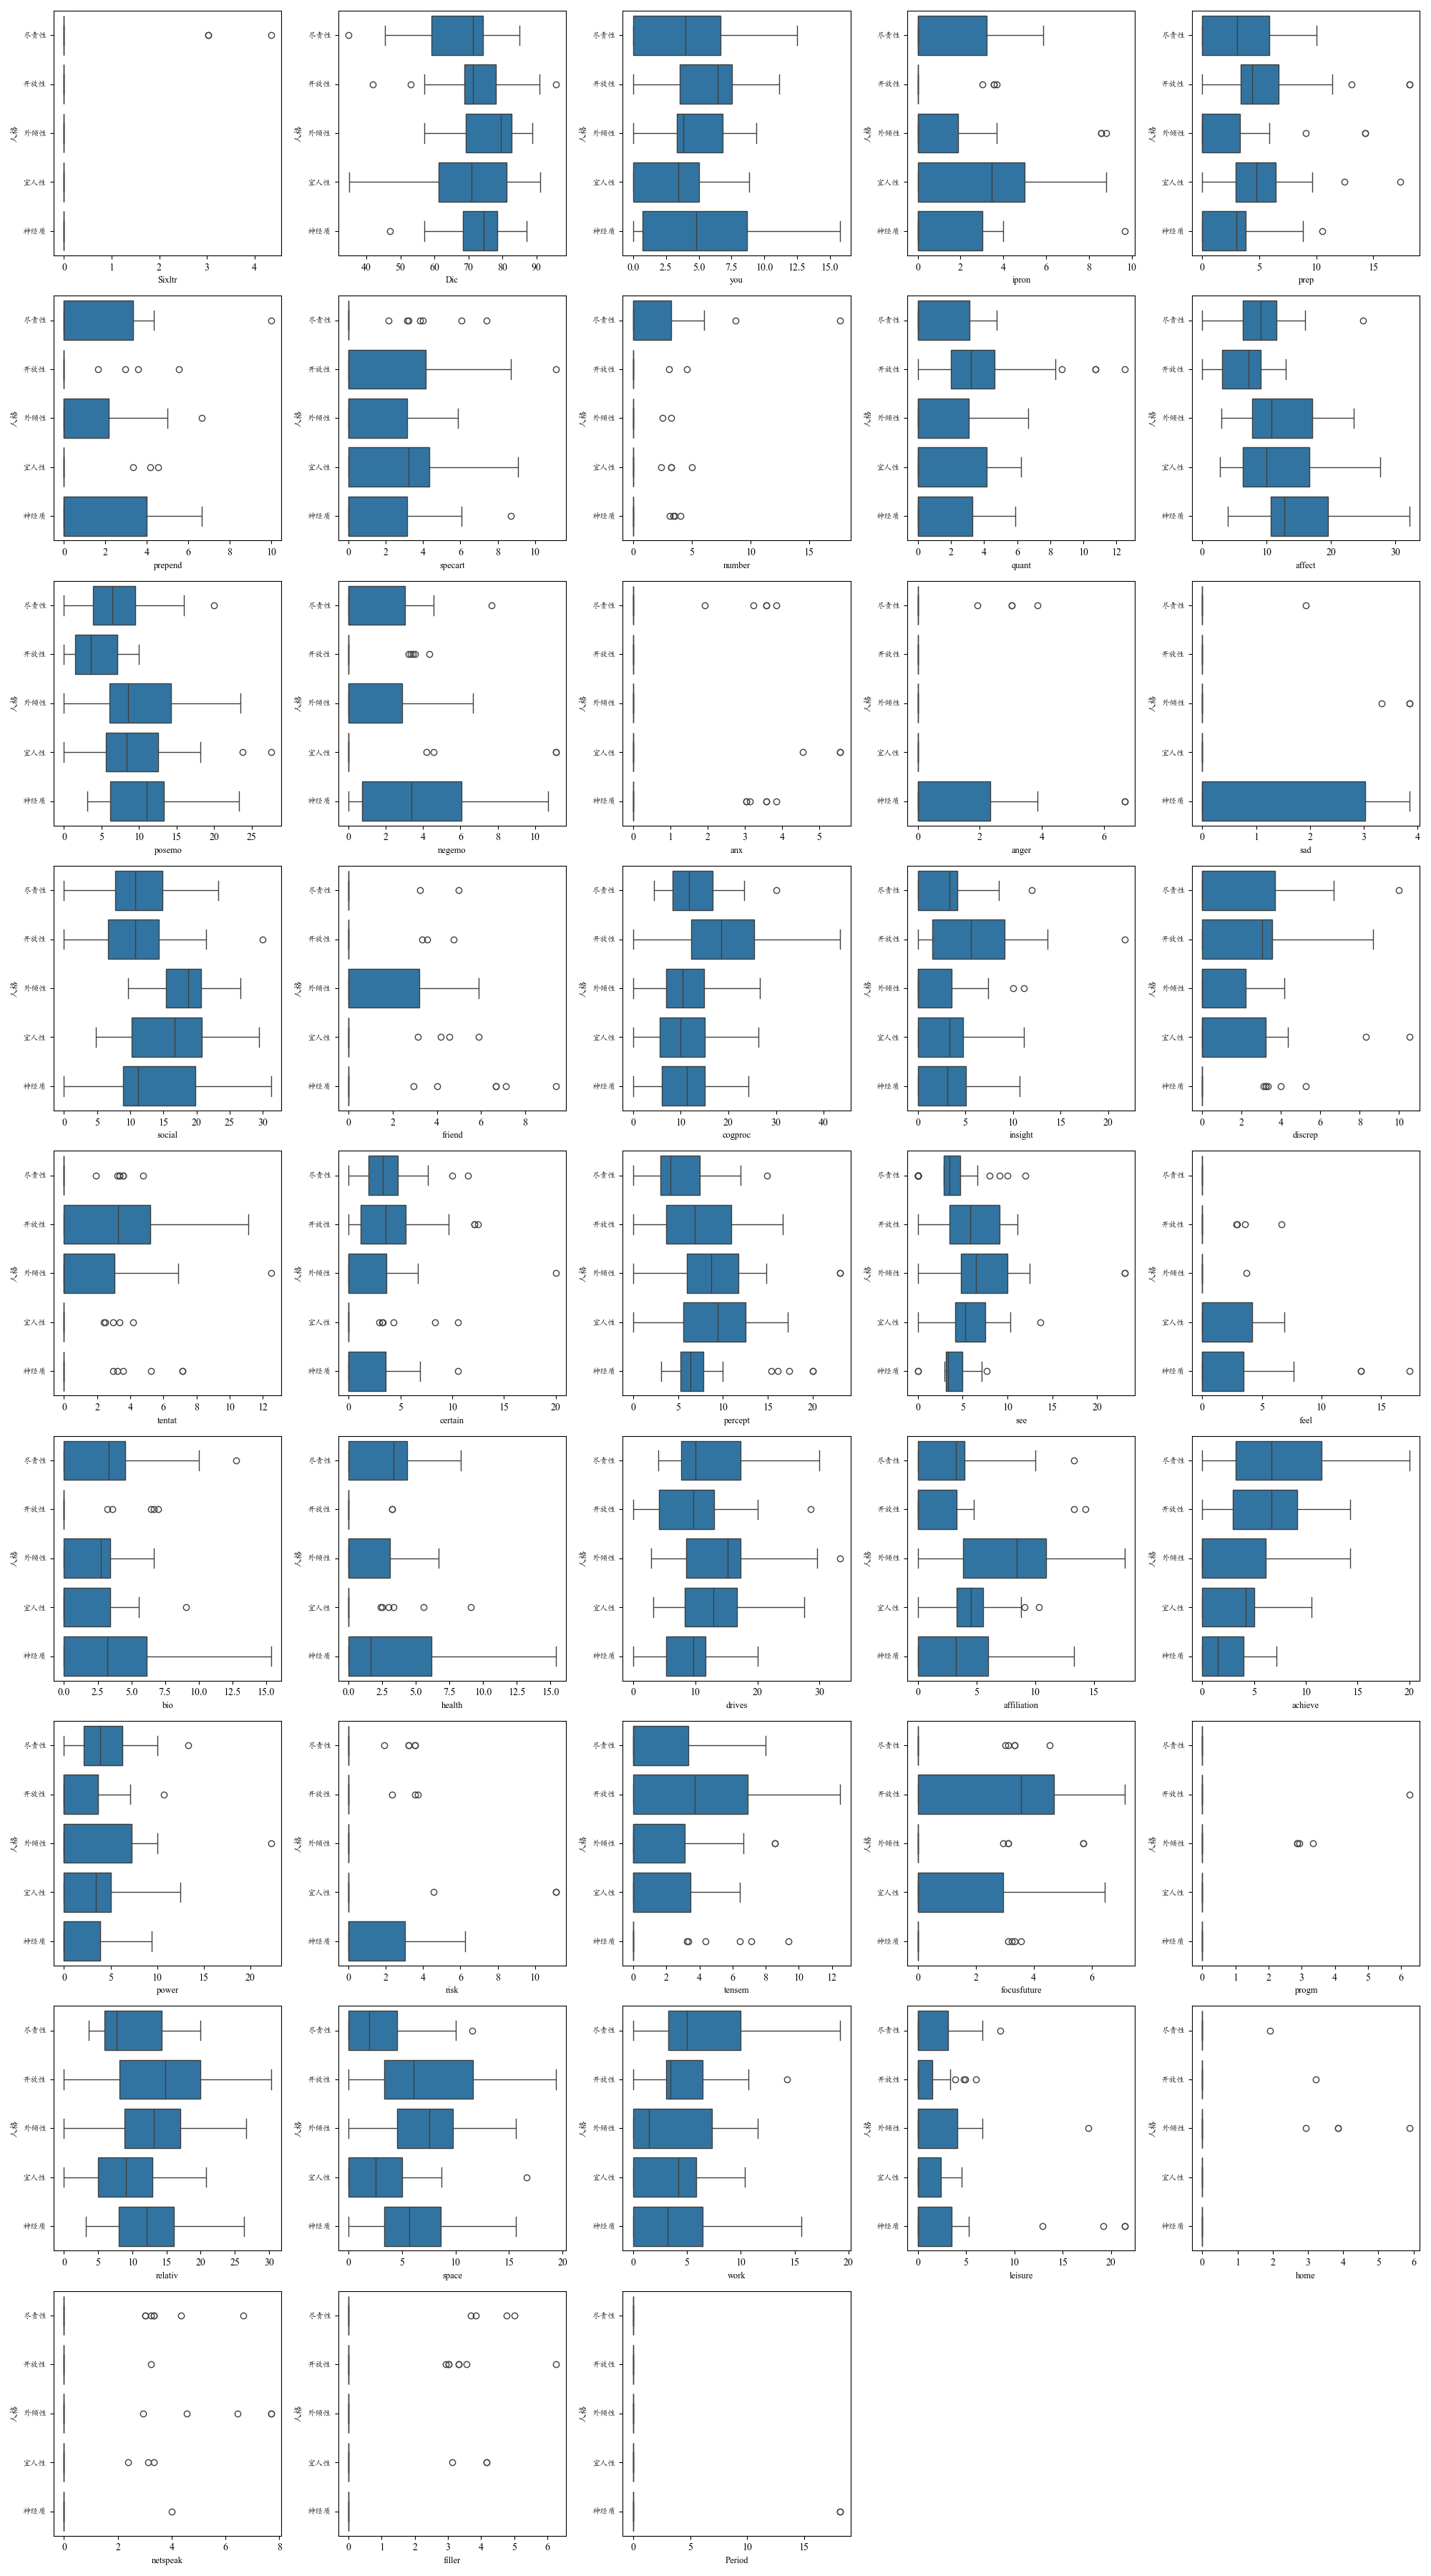
\includegraphics[width=0.8\linewidth]{Image/Study3-LIWC.png}
    \caption{\label{fig:Study3-LIWC}基于大五人格特质的个性化广告文本的语言特征分布}
\end{figure}

\textbf{外倾性}广告语言突出社交性与情感表达,符合外倾性人格的活跃与互动特质。外倾性广告中的社交相关词(social, \textit{F}(4,132) = 6.360, \textit{p} = 0.0001, 18.17\%)和归属动机词(affiliation, \textit{F}(4,132) = 9.840, \textit{p} < 0.001, 7.72\%)显著高于其他人格特质,体现出强烈的社交导向。此外,外倾性广告中的正面情感词(posemo, \textit{F}(4,132) = 7.181, \textit{p} < 0.001, 10.35\%)和感知词(percept, 9.32\%)的比例均为最高,进一步突出了积极、外向和注重体验的语言风格。

\textbf{宜人性}广告语言突出了情感温度和人际联结,体现了宜人性人格的共情与亲和特质。宜人性广告在正面情感词(posemo, 9.71\%)、社交相关词(social, 15.58\%)和归属动机词(affiliation, 4.75\%)方面均有较高占比,显示出广告内容偏向温暖、友好和关怀。此外,宜人性广告的语言风格也较为柔和,使用更多的情感相关词(affect, \textit{F}(4,132) = 8.942, \textit{p} < 0.001, 11.37\%)来增强情感连接。

\textbf{尽责性}广告语言风格注重目标导向和逻辑性,凸显了尽责性人格的计划性与成就驱动力。高尽责性广告中成就动机词(achieve, \textit{F}(4,132) = 6.710, \textit{p} = 0.0001, 7.32\%)使用最多,符合尽责性人格对成功和结果导向的关注。此外,尽责性广告在长词使用率(Sixltr, \textit{F}(4,132) = 2.898, \textit{p} = 0.0245)和数量词使用率(quant, \textit{F}(4,132) = 6.061, \textit{p} = 0.0002)上也显著高于其他特质,表现出语言上的正式性和条理性。

\textbf{开放性}广告文案呈现出鲜明的探索性与认知导向特征。高开放性广告在认知加工词(cogproc, \textit{F}(4,132) = 7.442, \textit{p} < 0.001, 19.60\%)和洞察词(insight, \textit{F}(4,132) = 3.829, \textit{p} = 0.0056, 5.93\%)的使用比例显著高于其他人格特质,反映了开放性人格偏好深入思考与探索的特质。此外,开放性广告大量使用空间相关词(space, \textit{F}(4,132) = 6.550, \textit{p} = 0.0001, 7.19\%)与感知词(percept, \textit{F}(4,132) = 3.321, \textit{p} = 0.0125, 7.74\%),表现出强调体验、探索与审美感知的语言风格。

\textbf{神经质}广告语言表现出显著的情绪波动与情感敏感特征。神经质广告中负面情感词(negemo, \textit{F}(4,132) = 7.308, \textit{p} < 0.001, 3.84\%)、焦虑词(anx, \textit{F}(4,132) = 2.845, \textit{p} = 0.0266, 0.78\%)、愤怒词(anger, \textit{F}(4,132) = 6.394, \textit{p} = 0.0001, 1.19\%)和悲伤词(sad, \textit{F}(4,132) = 8.058, \textit{p} < 0.001, 1.15\%)的使用均显著高于其他人格特质。这种情绪化的表达不仅强化了情感连接,也反映了神经质个体对情绪体验的高度敏感性。


在 LIWC 分析基础上,我们进一步通过词云图(图 \ref{fig:Study3-wordCloud})展示了五种人格特质广告的高频词。在制作词云图时,为突出各人格特质广告在语言风格上的差异,我们首先对五种人格个性化广告文本进行了预处理。具体而言,剔除了广告文本中未能体现人格特征且具有广泛通用性的高频词,例如“手机”“我们”“智能”等通用词汇。这些词语虽在广告中频繁出现,但主要源于广告语境和产品描述,与人格特质无直接关联,保留反而会掩盖不同人格特质在语言特征上的差异性。词云图中词语的大小代表其在对应人格广告中的出现频率,直观反映了各人格特质广告在语言风格上的差异。针对\textbf{外倾性}的广告,突出社交体验与分享感,词云中高频词如\textbf{“世界”“朋友”“分享”}与LIWC 中社交词(social)类别的高频结果一致,充分体现了外倾性个体偏好社交和互动的特质。\textbf{宜人性}广告强调情感共鸣与温暖体验,\textbf{如“美好”“温暖”“陪伴”}与 LIWC 中积极情感词(posemo)类别的高频结果相符,符合宜人性人格重视人际和情感连接的特点。\textbf{尽责性}广告则突出了功能性和可靠性,词云中的\textbf{“精准”“高效”“细节”}与 LIWC 中成就动机词(achieve)和认知加工词(cogproc)类别一致,契合尽责性人格偏好条理性和目标导向的特征。\textbf{开放性}广告则体现了探索与创造性的主题,高频词如\textbf{“创意”“探索”“无限”}与 LIWC 中感知类(percept)和洞察类词(insight)的高频结果相符,反映了开放性人格追求新体验和创造力的偏好。\textbf{神经质}广告则着重于情感安抚与安全感,\textbf{“陪伴”“温暖”“放松”}如,与 LIWC 中负面情感词(negemo)、焦虑词(anx)及亲和性词(affiliation)的显著性结果一致,突出了神经质人格在情绪波动中对安全感和情感支持的需求。

综合 LIWC 分析与词云可视化结果,本研究揭示了不同人格特质广告在语言特征上的显著差异,充分展现了基于大五人格模型的个性化广告语言模式。这一结果不仅丰富了对个性化广告语言特征的理解,也进一步验证AI基于人格特征生成个性化广告文本的能力。

\begin{figure}[H]
    \centering
    % 第一行三张图
    \subfloat[外倾性]{
        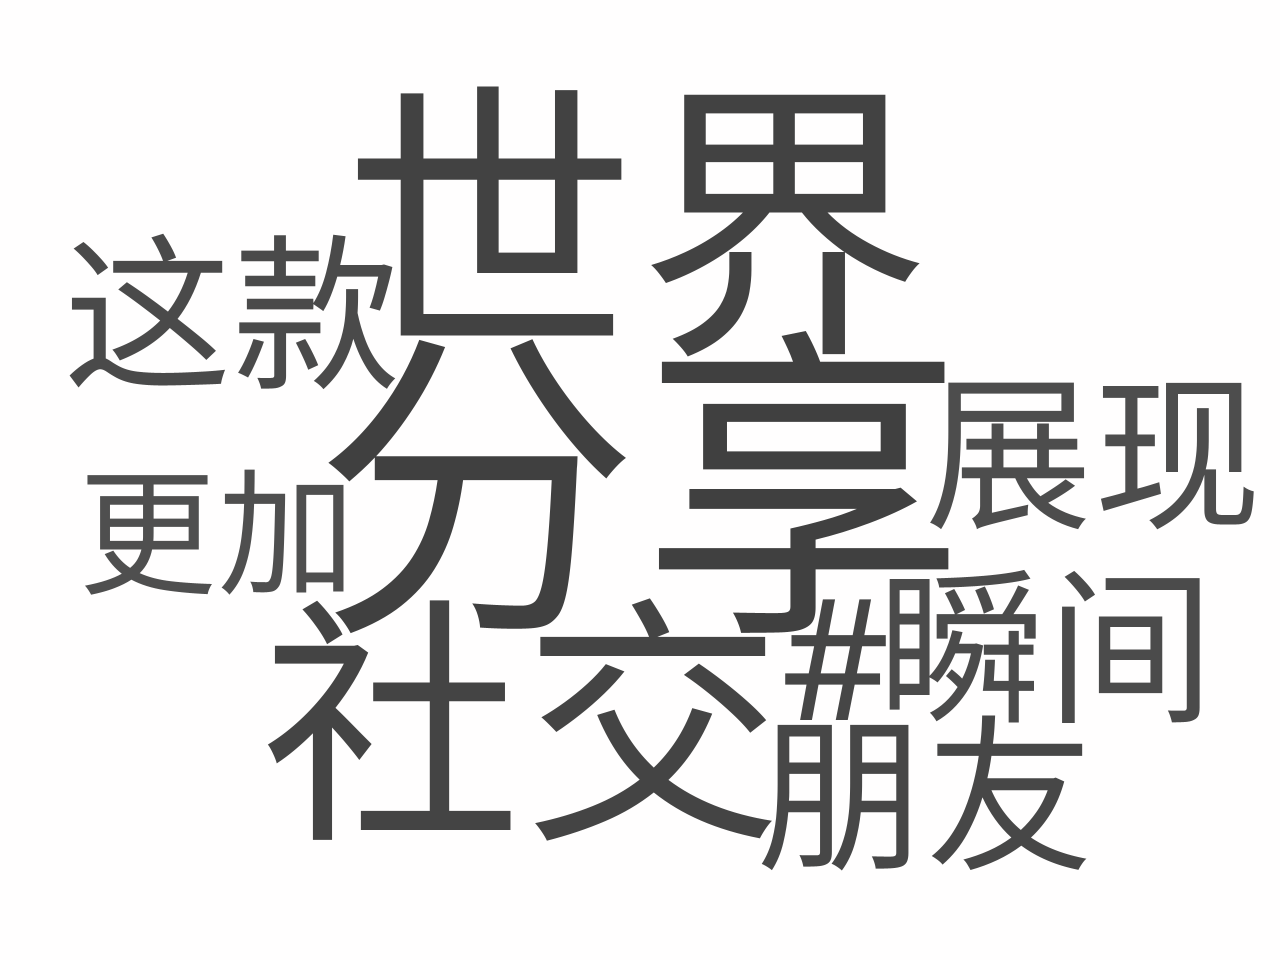
\includegraphics[width=0.2\linewidth]{Image/Study3-外倾性.png}
    }\hspace{1em}
    \subfloat[宜人性]{
        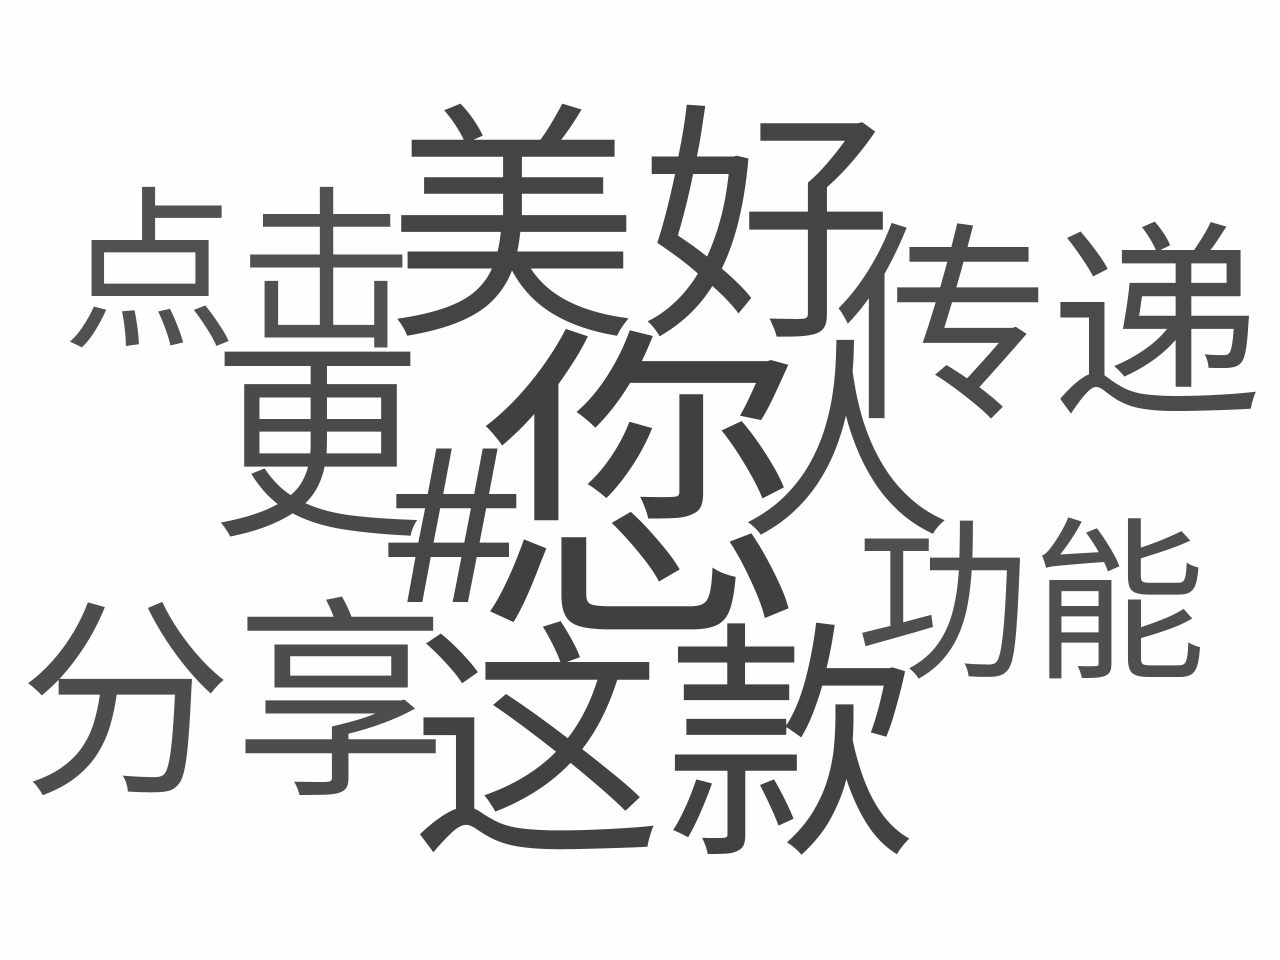
\includegraphics[width=0.2\linewidth]{Image/Study3-宜人性.png}
    }\hspace{1em}
    \subfloat[尽责性]{
        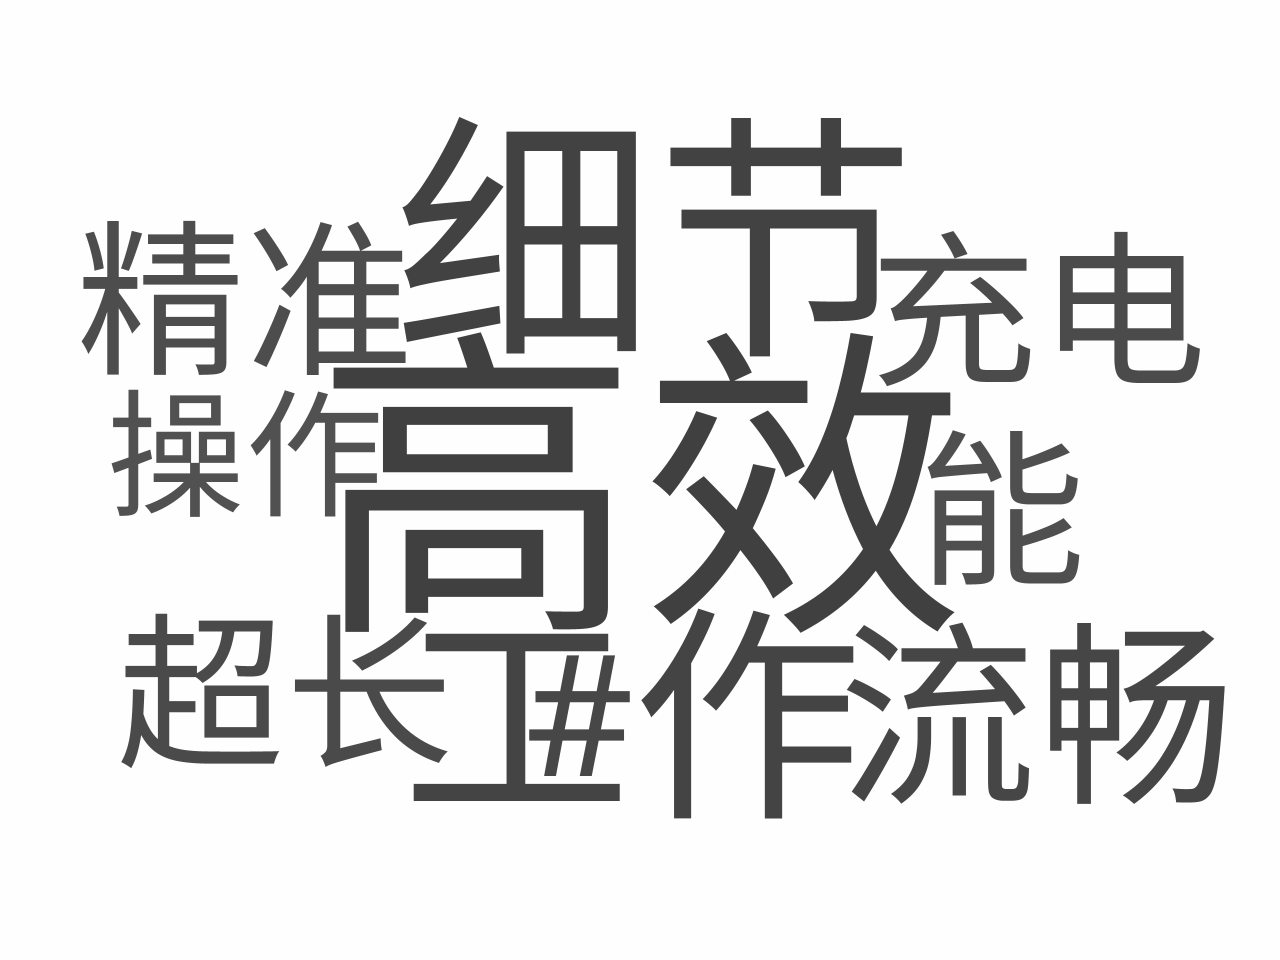
\includegraphics[width=0.2\linewidth]{Image/Study3-尽责性.png}
    }
    \\[1em] % 换行并增加垂直间距
    % 第二行两张图
    \subfloat[开放性]{
        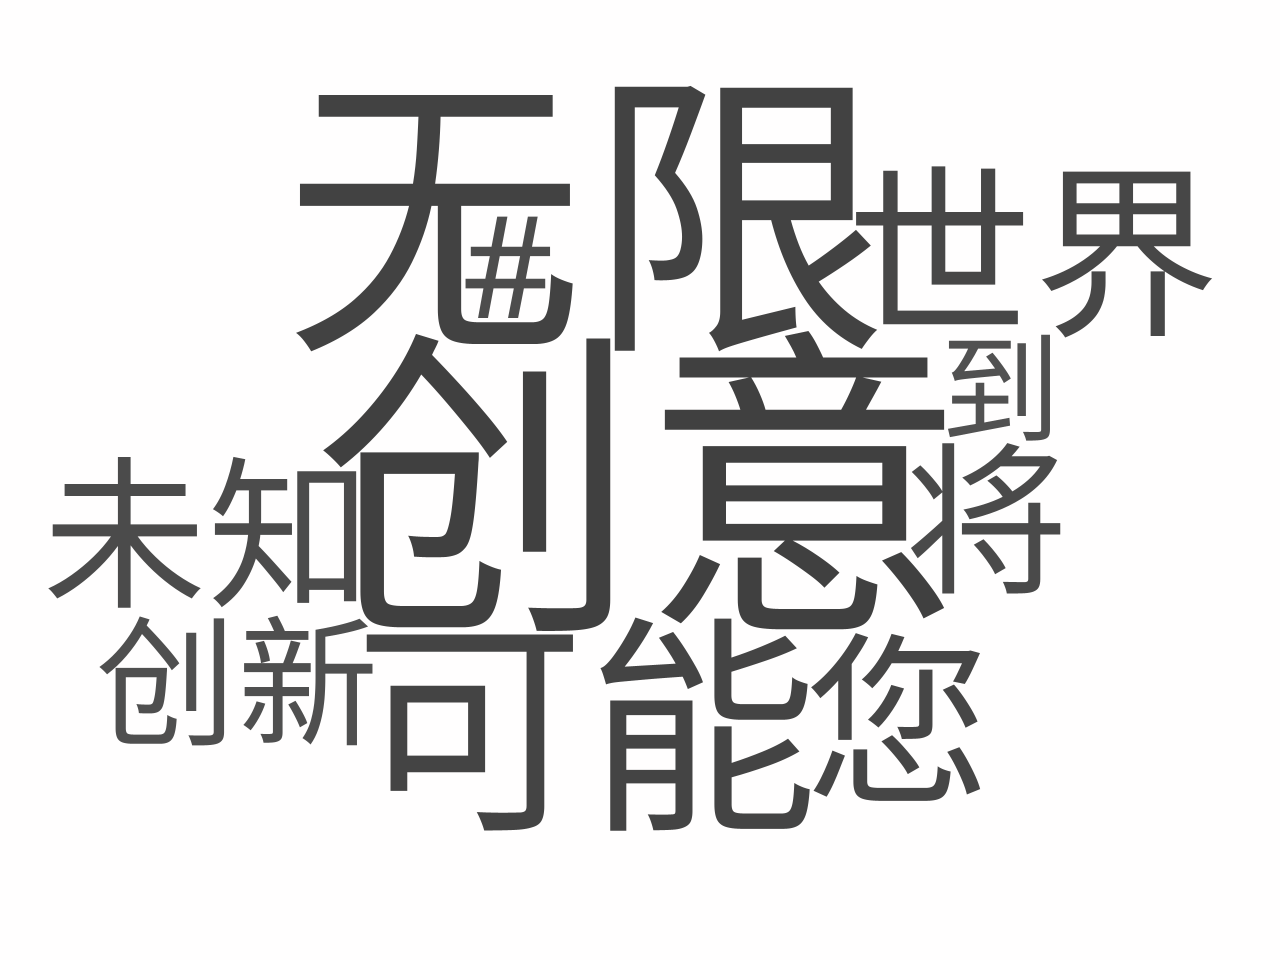
\includegraphics[width=0.2\linewidth]{Image/Study3-开放性.png}
    }\hspace{2em}
    \subfloat[神经质]{
        
\includegraphics[width=0.2\linewidth]{Image/Study3-神经质.png}
    }
    \caption{\label{fig:Study3-wordCloud}基于大五人格特质的个性化广告文本词云图}
    \label{fig:personality_images}
\end{figure}

